% 원문 2.3절(손실 압축) ~ 2.4.2절(점진적 정밀화), PDF 11--20쪽
\subsection{손실 압축}

손실 압축의 핵심 문제는 압축률 제약 아래에서 복원 기준을 만족하도록 대상을 표현하는 일이다.
채널 부호화나 거의 무손실 압축에서는 블록 오류율을 성능 지표로 삼는다.
반면 손실 압축은 기호 오류율로 평가할 수 있다 [14].

\subsubsection{비점근 한계}

무손실 압축에서 식 (6)으로 정의한 정보 확률변수에 착안하여, 손실 압축의 비점근 이론에서는 $\dd$-기울인 정보(d-tilted information) [10]라는 양을 중요하게 다룬다.
이 양을 바탕으로 역 한계와 달성 가능성 한계를 모두 얻을 수 있다.
먼저 그 정의는 다음과 같다.
\begin{equation}
  \ttl_S(s,d) = \log \frac{1}{\E\left[\exp\left\{\lambda^\star d - \lambda^\star \dd(s,Z^\star)\right\}\right]},
  \tag{8}
\end{equation}
이 양은 본질적으로 원천 출력 $s$를 왜곡 $d$ 이내로 표현하는 데 필요한 비트 수를 나타낸다.
라그랑주 승수(Lagrange multiplier)는 $\lambda^\star = -\mathbb{R}_S'(d)$이고, 정보 율-왜곡 함수는 $\mathbb{R}_S(d) = \E[\ttl_S(S,d)]$이다.
$d=0$이고 이산 확률변수에 대해 $\dd(s,z)=\mathbf{1}\{s\neq z\}$이면 0-기울인 정보를 $\ttl_S(s,0)$으로 정의하면 자연스럽다.
이 양은 거의 무손실인 경우에 식 (6)의 정보 확률변수 $\iinf_S(s)$로 환원된다.
또한 긴 수열은 평균에 가까워지는 경향이 있다는 직관에 따라, $\ttl_{S^k}(S^k,d)$의 평균값은 점근적 최적 부호율 $kR(d)$와 같다\footnote{간단히 하기 위해 이하에서는 최소 달성 가능 부호율의 위 첨자를 생략한다.}.
여기서 점근적 근본 한계 $R(d)$는 부호 길이 $k$가 무한대로 갈 때 $R(k,d,\epsilon)$의 상한(supremum)이다. 즉 $R(d)=\sup_{k\to\infty} R(k,d,\epsilon)$이다\onote{원문 표기 그대로 옮겼다. $\sup_{k\to\infty}$는 관례적이지 않은 표기이며, $R(d)=\lim_{k\to\infty}R(k,d,\epsilon)$(극한)으로 읽는 것이 맞다.}.
$R(k,d,\epsilon)$은 비점근 영역에서 최소 부호책 크기 $M^\star(k,d,\epsilon)$에 대응하는 부호율이다.
촘촘한 비점근 한계는 두 확률을 서로 잇는다.
하나는 표현점이 $M$개인 부호의 왜곡이 $d$를 넘을 확률(조작적 양)이고, 다른 하나는 $\dd$-기울인 정보가 $\log M$을 넘을 확률(정보이론적 양)이다.
이 두 양은 점근 영역의 분류와 짝을 이룬다.
점근 영역에서는 달성 가능한 율-왜곡 쌍을 조작적 관점에서, 율-왜곡 함수를 정보적 관점에서 정의한다.

\paragraph{1) 역 한계}
Shannon은 [75]에서 평균 왜곡 기준 부호화의 근본 율-왜곡 한계를 확립했다.
이후 Körner 등 [76]과 Kieffer [77]는 손실 원천 부호화의 강한 역정리 한계를 증명했다.
이 결과에 따르면 고정 압축률 $R$이 $R<\mathbb{R}_S(d)$를 만족할 때 $k\to\infty$이면 오류 확률 $\epsilon$은 1로 간다.
접두 조건을 만족하는(prefix-free) 가변 길이 손실 압축에 대해서는 Kontoyiannis가 [16]에서 핵심적인 비점근 역 한계를 유도했다.
유한 알파벳 이산 무기억 원천과 유계이고 분리 가능한(separable) 왜곡 척도에 대해서는 Martons의 고정율 오류 지수 [17]로부터 유한 부호 길이 역 한계를 얻을 수 있다\onote{``Martons''는 ``Marton's''(Marton의)의 오기로 보인다.}.
이후 Han [18]과 Iriyama [19]는 오류 지수 분석 방법을 확장해 비점근 이론 결과를 얻었다.
$\dd$-기울인 정보로 역 한계를 얻는 방법 외에, [10]은 [11]에서 착안해 이진 가설 검정에 기반한 한계도 얻었다. 이 한계는 경우에 따라 더 촘촘할 수 있다.
알파벳 $\mathcal{S}$ 위에 정의된 보조 분포를 $Q$라 하자.
그리고 출력 1이 참 원천 분포 $P_S$ 쪽을 택하는 임의의 무작위 검정 $P_{W|X}:\mathcal{S}\mapsto\{0,1\}$을 생각하자.
이 접근으로, 주어진 충실도 기준을 만족하는 임의의 부호의 크기 $M$에 대해 다음 하한을 얻는다\footnote{$P$와 $Q$는 분포를 나타내고, $\P$와 $\Q$는 바탕 공간에서 사건의 확률을 나타낸다.}.
\begin{equation}
  M \ge \sup_{Q} \inf_{z\in\mathcal{Z}} \frac{\beta_{1-\epsilon}(P_S,Q)}{\Q\left[\dd(S,z)\le d\right]},
  \tag{9}
\end{equation}
관측된 원천 출력 $s\in\mathcal{S}$에 대해 이진 가설 검정의 최적 성능을 다음과 같이 정의한다.
\[
  \beta_\alpha(P,Q)\triangleq\min_{P_{W|X}:\P[W=1]\ge\alpha}\Q[W=1].
\]
원천 $S$가 가산 알파벳 $\mathcal{S}$에서 값을 취하고 분포 $Q$가 $\mathcal{S}$ 위의 균등 분포라고 하자.
이렇게 고르면 식 (9)보다 느슨한 하한이 나오지만, 한계의 의미를 이해하기는 더 쉽다.
확률 측도가 $1-\epsilon$인 집합 $\Omega\subset\mathcal{S}$를 생각하자.
임의의 $s\in\Omega$에 대해, 오류 확률이 $\epsilon$인 최적 이진 가설 검정은 $Q$ 대신 $P_S$를 택한다.
따라서 제2종 오류 $\beta_{1-\epsilon}(P_S,Q)$는 $\Omega$의 원소 개수에 비례하고, $\Q[\dd(S,z)\le d]$는 반지름 $d$인 왜곡 공 하나에 담을 수 있는 원소 개수에 비례한다.
그러므로 이 비는 집합 $\Omega$를 덮는 데 필요한 왜곡 공의 최소 개수에 대한 하한이 된다.
다만 왜곡 $\dd$-공끼리 겹치기 때문에 이 하한은 흔히 달성되지 않는다.

\paragraph{2) 달성 가능성 한계}
가장 일반적인 달성 가능성 한계는 오류 확률의 상한을 보장하는 부호가 존재함을 말해 준다.
이 한계는 Shannon [75]에서 비롯되었고, 이후 Verdú가 [78]에서 정제했다.
독립 동일 분포(i.i.d., independent and identically distributed) 원천과 분리 가능한 왜곡 척도를 갖춘 세 가지 구체적 설정에 대해서도 달성 가능성 한계가 알려져 있다.
Goblick은 유한 알파벳 원천의 고정율 압축 [79], Pinkston은 유한 알파벳 원천의 가변율 압축 [80], Sakrison은 평균 제곱 오차 왜곡 아래 가우스 원천의 가변율 압축 [81]에 대해 각각 달성 가능성 한계를 제시했다.
그러나 이 한계는 어느 정도 다루기 번거로운 경우가 많다.
이후 Kostina 등 [10]은 달성 가능성 한계를 얻는 두 가지 주요 접근을 개발했다.
두 접근은 앞서 소개한 무손실 압축의 비점근 근본 한계 분석 방법에서 착안한 것이다.
첫째 접근은 무작위 부호화로 원천 출력을 부호화한다.
이때 초과 왜곡 확률은 $M$개의 부호어 중 어느 것도 원천 출력 $s$를 중심으로 한 반지름 $d$의 왜곡 공 안에 들어가지 않는 사건에서 나온다.
실제로 이 접근은 계산 복잡도가 높아 수치적으로 평가하기가 다소 어렵다.
둘째 접근은 (일반화된) $\dd$-기울인 정보를 이용해, 부호어가 $s$ 주위의 왜곡 공 안에 들어갈 확률의 하한을 유도한다.
이 방법에서는 왜곡 $\dd$-공 표면의 구면 껍질 반지름을 반영하는 매개변수 $\gamma$를 도입한다.
이 기법은 무작위 부호화 방법의 한계를 분석할 때 특히 유용하다.

\subsubsection{근사}

가변율 양자화에서 손실 AEP(점근적 등분배 성질, asymptotic equipartition property)는 강력한 달성 가능성 한계와 역 한계를 낳으며, 왜곡 $\dd$-공의 점근적 거동을 다룬다.
손실 AEP의 2차 정밀화는 Yang 등 [20]과 Kontoyiannis [16]가 연구했다.
이후 Kostina 등 [10]은 상당히 일반적인 조건 아래에서 임의 알파벳 원천의 최소 달성 가능 부호율에 대한 점근 근사를 유도했다.
이 결과는 촘촘한 비점근 한계와 손실 AEP의 비점근 정밀화를 적용해 얻은 것이다.

[10]의 가우스 근사를 소개하기 전에, 몇 가지 조건이 필요하다.
먼저 원천 $\{S_i\}$는 정상(stationary)이고 무기억이라고 가정한다. 왜곡 척도는 분리 가능해야 하며, 왜곡 수준은 적절히 유계여야 한다.
또한 확률변수 $\dd(S,Z^\star)$의 9차 적률이 유한해야 한다. 여기서 $Z^\star$는 율-왜곡 함수를 달성하는 복원이다.
이 조건 아래에서 최소 달성 가능 부호율은 다음을 만족한다.
\begin{equation}
  R(k,d,\epsilon) = R(d) + \sqrt{\frac{\mathcal{V}(d)}{k}}\,Q^{-1}(\epsilon) + \theta\left(\frac{\log k}{k}\right),
  \tag{10}
\end{equation}
여기서 1차 항 $R(d)$와 2차 항 $\mathcal{V}(d)$는 각각 $\dd$-기울인 정보의 평균과 분산이다. 즉 $R(d)=\E[\ttl_{\mathsf{S}}(\mathsf{S},d)]$, $\mathcal{V}(d)=\Var[\ttl_{\mathsf{S}}(\mathsf{S},d)]$이다.
나머지 항 $\theta\left(\frac{\log k}{k}\right)$는 다음을 만족한다.
\begin{equation}
  -\frac{1}{2}\frac{\log k}{k} + O\left(\frac{1}{k}\right)
  \le \theta\left(\frac{\log k}{k}\right)
  \le C_0\frac{\log k}{k} + \frac{\log\log k}{k} + O\left(\frac{1}{k}\right),
  \tag{11}
\end{equation}
여기서 $C_0 = \frac{1}{2} + \frac{\Var\left(J'_{Z^\star}(\mathsf{S},\lambda^\star)\right)}{\E\left[\left|J''_{Z^\star}(\mathsf{S},\lambda^\star)\right|\right]\log e}$이고 $\lambda^\star=-\mathbb{R}_S'(d)$이다.
식 (10)의 근사는 유한 부호 길이 영역에서 최소 압축률이 율-왜곡 함수에서 얼마나 벗어나는지를 정량적으로 보여 준다.
첫째 항은 점근적 율-왜곡 함수에 해당하고, 나머지 항은 유한 부호 길이 제약 때문에 생기는 벌점 항으로 해석할 수 있다.
특히 주된 관심 대상은 2차 항이다.
2차 항은 $\dd$-기울인 정보의 분산과 초과 왜곡 확률 문턱값 $\epsilon$에 명시적으로 의존하며, 가우스 근사에서 $Q^{-1}(\cdot)$ 함수가 나온다.
식 (11)의 나머지 항은 $k$에 대한 차수까지는 확립되었지만, 더 날카로운 한계를 얻는 일은 아직 열린 문제로 남아 있다.

이 일반적 결과는 이진 무기억 원천(BMS, binary memoryless source), 이산 무기억 원천(DMS, discrete memoryless source), 가우스 무기억 원천(GMS, Gaussian memoryless source)에 적용되었으며, 오류 확률과 부호책 크기의 한계, 최소 달성 가능 압축률의 근사에 대한 시뮬레이션 결과도 함께 제시되었다.
예를 들어 GMS에서는 $\dd$-기울인 정보 $\ttl_{S^k}(s^k,d)$의 식을 유도할 수 있다.
여기서 $S^k\sim\mathcal{N}(0,\sigma^2)$은 길이 $k$인 i.i.d.\ 가우스 원천이고, $Z^{k\star}\sim\mathcal{N}(0,\sigma^2-d)$는 최적 복원 원천이다.
가설 검정에 기반한 역 한계에서는 가우스 원천에 대한 보조 분포 $\Q$로 르베그 측도(Lebesgue measure)를 흔히 쓰며, 이 선택이 효과적이다.
무작위 부호화에 기반한 달성 가능성에서는 가우스 원천의 구면 대칭성 덕분에 무작위 부호화가 고전적인 구 덮기 문제와 밀접하게 연결된다.
근사 부분에서는 $\ttl_{S^k}(s^k,d)$의 분포가 명시적으로 주어지므로 2차 분산 항 $\mathcal{V}(d)$를 쉽게 구할 수 있다.
나머지 항의 한계에 대한 자세한 내용은 [10, 14]를 참고하라.

\subsubsection{가우스-마르코프 원천}

앞에서는 무기억 원천을 소개했다 [10, 75].
그러나 이미지나 동영상 같은 실제 원천 상당수는 기억이 있으며, 화소 수준과 프레임 수준 모두에서 상관을 보인다 [82, 83].
따라서 기억이 있는 원천으로 연구를 확장하는 일이 중요하다.
무기억 원천과 달리, 기억이 있는 원천에 대한 촘촘한 결과는 대부분 초기에는 제한적이었고 점근 영역에서만 얻어졌다 [13].
Kolmogorov는 [84]에서 이차 왜곡 척도 아래 정상 가우스 자기회귀 원천의 율-왜곡 함수를 처음 유도했다.
이어 Berger는 [85]에서 이 결과를 비정상인 경우, 즉 위너 과정(Wiener process)으로 일반화했다.
Gray는 이후 [21]에서 이를 일반 가우스 자기회귀 원천과 1차 이진 대칭 마르코프 과정으로 확장했다.
기억이 있는 원천의 흔한 모형은 1차 마르코프 기억을 지닌 가우스 원천이다 [86].
이를 가우스-마르코프 원천(Gauss-Markov source)이라 하며, 가우스 자기회귀 원천의 특수한 경우이다 [21].
기억이 있는 원천의 비점근 근본 한계에서 주된 진전은 Tian 등이 이루었다.
이들은 정상 가우스-마르코프 원천을 [22]에서, 비정상인 경우를 [23]에서 분석했다.
여기서는 정상인 경우를 예로 들어, 비점근 달성 가능성 한계와 역 한계, 근사를 유도하는 과정을 소개한다.
이 예에서 가우스-마르코프 원천의 비점근 근본 한계를 얻는 핵심 방법을 살펴본다.

가우스-마르코프 원천은 모든 $i\ge 1$에 대해 다음과 같이 모형화할 수 있다.
\begin{equation}
  U_i = aU_{i-1} + Z_i,
  \tag{12}
\end{equation}
여기서 $U_0=0$이고, $Z_i$는 $Z_i\sim\mathcal{N}(0,\sigma^2)$인 i.i.d.\ 가우스 확률변수이다.
$|a|<1$, $|a|>1$, $|a|=1$은 각각 정상 원천, 비정상 원천, 위너 과정에 해당한다.
[22]에서는 원래 [10]이 GMS에 대해 정의한 $\dd$-기울인 정보 $\ttl_{X^k}(x^k,d)$를 가우스-마르코프 원천으로 확장했다. 이 확장에는 역 물 채우기 원리가 자연스럽게 녹아 있다.

\paragraph{1) 역 한계}
역 한계를 얻는 주된 방법은 두 가지이다.
하나는 부피 논증(volumetric argument)에, 다른 하나는 $\dd$-기울인 정보에 기반한다.
부피 논증은 가우스 분포의 구면 대칭성 덕분에 성립한다.
부호어 공간에서 왜곡 $\dd$-공은 상관 때문에 특정 축을 따라 늘어나거나 줄어들어 타원체로 바뀔 수 있다.
그러나 상관은 원천의 에너지를 바꾸지 않으므로 전체 부피는 변하지 않는다.
따라서 역 한계는 본질적으로 i.i.d.\ 가우스 경우와 같다.
다만 i.i.d.\ 가우스 경우와 달리, 가우스-마르코프 원천에서 부피 방법은 저왜곡 영역에서만 최적 2차 부호율을 줄 수 있다 [22, Theorem 7].
더 일반적인 접근은 여전히 상관을 제거한(decorrelated) 원천의 $\dd$-기울인 정보에 의존한다. 자세한 내용은 [22]를 참고하라.

\paragraph{2) 달성 가능성 한계}
Dumer 등 [87]은 $\mathbb{R}^k$의 타원체를 최소 개수의 공으로 덮는 문제를 연구하고, 덮개 수(covering number)의 하한과 상한을 모두 유도했다.
그러나 구 덮기 기법에서 착안해 [87]의 결과를 가우스-마르코프 원천의 최소 달성 가능 부호율에 대한 달성 가능성 한계에 그대로 적용하면, 매우 느슨한 결과가 나온다.
구면 균일성이 사라지고 왜곡 $\dd$-공에 선형 변환(즉 상관 제거)이 가해지면서 타원체의 덮개 수가 크게 달라지기 때문이다.
달성 가능성 한계를 얻는 더 믿을 만한 접근은 최대 우도 추정량에 기반해 전형 집합(typical set)을 구성하는 것이다. 이 접근은 가우스-마르코프 원천의 손실 AEP에 의존한다 [22].

\paragraph{3) 근사}
가우스-마르코프 원천의 최소 달성 가능 부호율은 다음을 만족한다 [22, Theorem 1].
\begin{equation}
  R(k,d,\epsilon) = \mathbb{R}_U(d) + \sqrt{\frac{V_U(d)}{k}}\,Q^{-1}(\epsilon) + o\left(\sqrt{\frac{1}{k}}\right),
  \tag{13}
\end{equation}
여기서 $\mathbb{R}_U(d)$는 율-왜곡 함수이다.
2차 항에서 조작적 분산도는 다음과 같다.
\begin{equation}
  V_U(d) = \frac{1}{4\pi}\int_{-\pi}^{\pi} \min\left\{1, \left(\frac{S(w)}{\theta}\right)^2\right\} dw,
  \tag{14}
\end{equation}
여기서 $\theta>0$은 왜곡 $d$에 대응하는 수위이고, 전력 스펙트럼은 $S(w)=\frac{\sigma^2}{g(w)}$, $g(w)=1+a^2-2a\cos(w)$로 정의한다.

\subsubsection{불일치}

불일치(mismatch) 문제는 손실 데이터 압축에서 생기는 실제적 난제에서 비롯된다.
어떤 분포의 원천에 맞춰 설계한 부호책을, 분포가 다른 원천을 압축하는 데 쓰는 상황이다.
다시 말해 압축할 원천이 미리 설계한 부호책과 맞지 않는다.
Lapidoth는 [24]에서 이차 왜곡 척도 아래 임의의 무기억 원천을, 구면 부호책과 최소 유클리드 거리 부호화로 압축했다.
Lapidoth의 결론은 다음과 같다. 2차 적률 $\sigma^2$이 유한하고 알려져 있는 임의의 에르고딕 원천에 대해, 분포가 $\mathcal{N}(0,\sigma^2)$인 GMS의 율-왜곡 함수는 부호 길이가 커질 때 달성 가능하며 앙상블 관점에서 tight(앙상블 tight, ensemble tight)하다.
앙상블 tight란 부호 앙상블 분석이 최적이라는 뜻이다.
주목할 점은, Lapidoths의 연구가 원천의 2차 적률만 요구하기 때문에 불일치 문제의 해결을 진전시켰다는 것이다\onote{``Lapidoths''는 ``Lapidoth's''의 오기로 보이며, 아래에서도 같다.}.
2차 적률은 원천 분포 전체보다 얻기 쉽고, 관측한 원천 수열로부터 추정할 수 있다.
이후 Zhou 등 [25]은 이 결과를 두 가지 부호책 유형으로 확장했다.
하나는 구면 부호책으로, 각 부호어를 반지름 $\sqrt{k(\sigma^2-d)}$인 구의 표면에서 독립적이고 균일하게 생성한다.
다른 하나는 가우스 부호책으로, 각 부호어를 평균 0, 분산 $\sigma^2-d$인 곱 가우스 분포에서 뽑는다.
원천 분포가 알려진 경우와 달리, 이때 성능은 원천 분포와 부호책 분포 모두에 대해 계산한 앙상블 초과 왜곡 확률로 평가한다.
Zhou 등 [25]은 최소 달성 가능 부호율의 2차 근사를 유도해 Lapidoth의 1차 점근 결과를 개선했다.
또한 Lapidoths의 연구를 서로 다른 두 유형의 부호책으로 확장했고, 두 부호책 모두 같은 1차 및 2차 최적성을 달성한다고 결론지었다.

$\E[S^2]=\sigma^2$, $\zeta=\E[S^4]<\infty$, $\E[S^6]<\infty$를 만족하는 임의의 무기억 원천 $S$에 대해, 주어진 부호책 유형 $\dagger\in\{\mathrm{sp},\mathrm{iid}\}$의 2차 근사는 다음과 같다 [25, Theorem 1].
\begin{equation}
  R^\dagger(k,\sigma^2,d,\epsilon) = \log\left(\frac{\sigma^2}{d}\right) + \sqrt{\frac{V(\sigma^2,\zeta)}{k}}\,Q^{-1}(\epsilon) + O\left(\frac{\log k}{k}\right),
  \tag{15}
\end{equation}
여기서 불일치 분산도는 $V(\sigma^2,\zeta)\triangleq\frac{\zeta-\sigma^4}{4\sigma^4}$로 정의한다.

직관적으로, 주된 오류 사건은 분포를 모르는 원천 수열이 비전형적(atypical)이라는 데서 생긴다.
그러나 두 부호책 유형 중 어느 것을 쓰든, 대략 $\exp\left(\frac{k}{2}\log\frac{\sigma^2}{d}\right)$개의 부호어면 모든 전형 수열을 덮기에 충분하며, 이때 오류 확률은 지수보다 빠르게 감소한다.
이 결과는 비전형 원천 수열의 확률을 세심하게 분석해 얻었다.
자세한 내용은 [25]를 참고하라.

\subsection{다중 단말 설정}

이제 다중 단말 설정으로 넘어간다.
여기서는 두 가지 주요 문제에 집중한다.
첫째 문제에서는 두 복호기가 하나의 공통 부호기의 출력을 복원한다.
부가 정보는 부호기와, 두 복호기 중 하나에서 모두 쓸 수 있다.
이 문제는 Kaspi가 [26]에서 처음 제기했으며, ``Kaspi 문제''라고도 부른다.
둘째 문제에서는 고전적인 율-왜곡 정식화에 부호기-복호기 쌍을 하나 더한다.
그 결과 부호기 둘과 복호기 둘로 이루어진 시스템이 되며, 이를 점진적 정밀화(successive refinement) 문제라 한다 [88].

\begin{figure}[t]
  \centering
  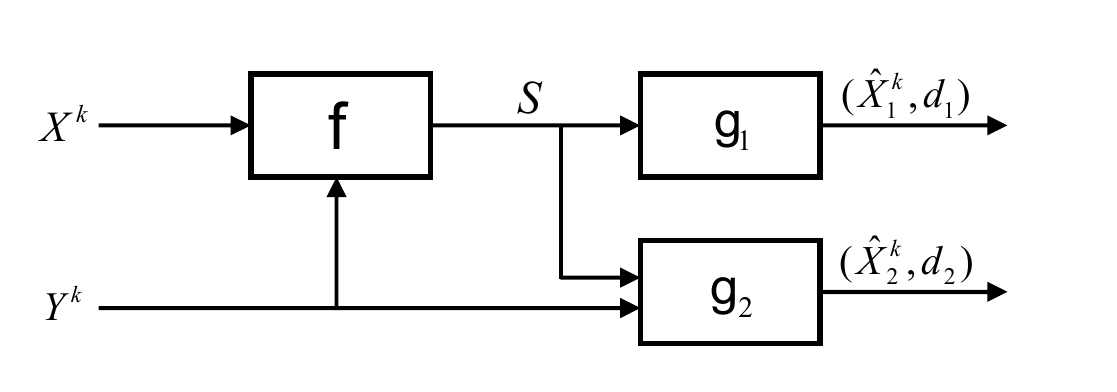
\includegraphics[width=0.85\linewidth]{fig/fig2.png}
  \caption{Kaspi 문제의 시스템 모형.}
\end{figure}

\subsubsection{Kaspi 문제}

Kaspi 문제의 모형은 그림~2와 같으며, 공통 부호기 $\ff$ 하나와 복호기 $\gg_i$ ($i=1,2$) 둘로 이루어진다.
부가 정보 $Y^k$는 $\gg_2$에서만 쓸 수 있다.
복호기 출력이 $\widehat{X}_i^k$ ($i=1,2$) 둘이므로, 서로 다른 왜곡 척도 두 개와 그에 대응하는 제약을 쓴다.
비점근 영역에서는 결합 초과 왜곡 확률
$P_{e,k}(d_1,d_2)\triangleq\P\left[\dd_1(X^k,\widehat{X}_1^k)>d_1 \text{ 또는 } \dd_2(X^k,\widehat{X}_2^k)>d_2\right]$
로 성능을 측정한다. 이 확률은 원천 분포와 부호책 분포를 모두 고려한다.
사실 [28]에서는 최적 부호의 성능을 평가하는 데 개별 초과 왜곡 확률을 썼다.
그러나 Zhou 등 [29]은 결합 초과 왜곡 확률이 개별 확률보다 여러 장점이 있다고 지적했다.
따라서 여기서는 결합 초과 왜곡 확률 기준에 기반한 결과에 집중한다.

[27]에서는 P2P $\dd$-기울인 정보를 Kaspi 문제의 $(\dd_1,\dd_2)$-기울인 정보로 확장했다.
$(\dd_1,\dd_2)$-기울인 정보의 핵심 성질 하나는, 원천과 부가 정보에 대한 기댓값이 율-왜곡 함수와 같다는 것이다. 즉 $R(P_{XY},d_1,d_2)=\E[\ttl_K(X,Y\mid d_1,d_2,P_{XY})]$이다.
Zhou 등은 $(\dd_1,\dd_2)$-기울인 정보의 이 성질과 Kostina 등의 단일 시행 역 논증 [89]을 바탕으로 Kaspi 문제의 역 한계를 유도했다 [27, Lemma 5].
달성 가능성 부분에서는 Kaspi 문제에 대한 형(type) 덮개 보조정리를 얻고, $(\dd_1,\dd_2)$-기울인 정보의 성질을 적절한 테일러 전개와 함께 활용했다.
Zhou 등은 Berry-Esséen 정리를 적용해 점근 근사를 유도했을 뿐 아니라, 대편차와 중편차를 이용해 DMS에 대한 오류 지수의 점근적 거동도 유도했다 [27, Sec.~III, Sebsec.~D].
여기서는 주로 Berry-Esséen 정리로 얻은 Kaspi 문제의 최적 2차 부호율을 소개한다.

\begin{figure}[t]
  \centering
  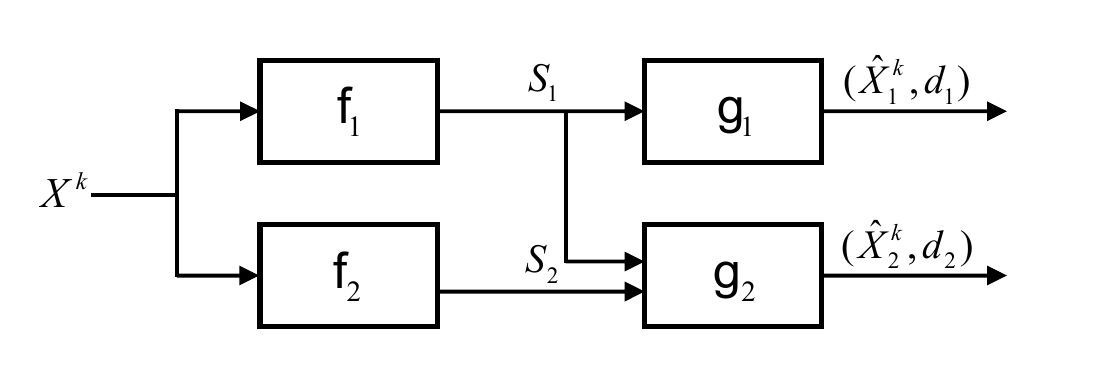
\includegraphics[width=0.85\linewidth]{fig/fig3.png}
  \caption{점진적 정밀화 문제의 시스템 모형.}
\end{figure}

Kaspi 문제의 왜곡-분산도 함수를 $V(d_1,d_2,P_{XY})$로 나타내자. 즉
\[
  V(d_1,d_2,P_{XY})=\Var\left[\ttl_K(X,Y\mid d_1,d_2,P_{XY})\right]
\]
이다.
부호율 $L$이 2차 $(d_1,d_2,\epsilon)$-달성 가능하다는 것은, 다음 두 조건을 만족하는 $(k,M)$-부호의 수열이 존재한다는 뜻이다.
\[
  \limsup_{k\to\infty}\frac{1}{\sqrt{k}}\left(\log M - k\,R(P_{XY},d_1,d_2)\right)\le L,
  \qquad
  \limsup_{k\to\infty}P_{e,k}(d_1,d_2)\le\epsilon.
\]
최적 2차 부호율은 이러한 달성 가능한 부호율 전체의 하한(infimum)으로 정의하고 $L^\star(d_1,d_2,\epsilon)$으로 나타낸다. 그 값은 다음과 같다.
\begin{equation}
  L^\star(d_1,d_2,\epsilon) = \sqrt{V(d_1,d_2,P_{XY})}\,Q^{-1}(\epsilon).
  \tag{16}
\end{equation}
덧붙여, 왜곡 수준 $(d_1,d_2)$에 따라 Kaspi 문제의 핵심 양 $\ttl_K(x,y\mid d_1,d_2,P_{XY})$는 다른 경우의 양으로 환원된다.
예를 들어 복호기 $\gg_2$를 없애면 Kaspi 문제는 통상적인 손실 원천 부호화 문제가 되고, $\ttl_K(x,y\mid d_1,d_2,P_{XY})$는 [10]의 $d_1$-기울인 정보로 환원된다.
마찬가지로 복호기 $\gg_1$을 없애면 부호기와 복호기 모두에서 부가 정보를 쓸 수 있는 경우가 되고, $\ttl_K(x,y\mid d_1,d_2,P_{XY})$는 [90]의 $d_2$-기울인 정보로 환원된다.

\subsubsection{점진적 정밀화}

점진적 정밀화 문제는 그림~3과 같다.
추가 복호기 하나가 두 부호기의 압축 출력에 동시에 접근한다 [88].
이 추가 복호기는 한 부호기에서만 정보를 받는 모형보다 원천 수열을 더 정밀하게 복원한다.
또한 점진적 정밀화 정식화는 다음 질문과 관련이 있다. 손실 압축의 최적성을 희생하지 않고도 전송을 중간에 끊었다가 특정 원천 수열을 더 잘 복원할 수 있는가 [30]?
Rimoldi는 [30]에서 임의의 왜곡 척도에 대해 DMS의 최적 율-왜곡 영역을 규명했다.
Effros는 이후 [31]에서 Rimoldi의 연구를 이산 정상 에르고딕 원천과 비에르고딕 원천으로 일반화했다.
Kanlis 등 [91]은 결합 초과 왜곡 기준 아래에서 오류 지수를 얻었고, Tuncel 등 [92]은 개별 초과 왜곡 기준을 다루었다.
No 등 [28]은 강한 점진적 정밀화 문제의 2차 부호율을 유도했다.
Zhou 등 [29]은 임의의 왜곡 척도를 지닌 DMS에 대해, 결합 초과 왜곡 기준 아래 점진적 정밀화 원천 부호화 문제의 최적 2차 부호율 영역과 중편차 상수를 유도했다.
이들은 이차 왜곡 척도를 쓰는 GMS도 다루었다. 이차 왜곡 척도 아래의 GMS는 점진적으로 정밀화 가능하므로 [88], 이 경우 결과가 특히 간단하다.

일반적인 DMS에서 율-분산도 행렬 $\mathbf{V}(R_1^\star,d_1,d_2\mid P_X)\succ 0$을 다음 2차원 확률벡터의 공분산 행렬로 두자.
\[
  \left[\,\ttl(X,d_1\mid P_X),\ \ttl(X,R_1^\star,d_1,d_2\mid P_X)\,\right]^T
\]
일정한 조건 아래에서 2차 부호율 영역은 [29, Theoremă11]에서 규명되었으며, 세 경우로 나뉜다\onote{``Theoremă11''은 조판 오류로, ``Theorem~11''로 읽는다. 문단 끝의 ``Theoremă6''도 ``Theorem~6''이다.}.
처음 두 경우에서는 부호의 부호율이 1차 한계 중 하나와 일정한 간격을 두고 떨어져 있으므로, 2차 거동을 일변량 가우스 분포로 포착할 수 있다.
반면 셋째 경우에서는 부호가 두 1차 한계에서 정확히 동작하므로, 2차 거동을 포착하려면 이변량 가우스 정식화가 필요하다.
이 결과는 Tan 등 [93, Theoremă6]의 논증에 따라 율-분산도 행렬이 양의 정부호인 경우와 계수 부족(rank-deficient)인 경우 모두에 성립한다.
